% !TeX root = ./main.tex
\documentclass[energies,article,submit,moreauthors,pdftex]{Definitions/mdpi} 
%----------
% submit/accept
%----------
% The class option "submit" will be changed to "accept" by the Editorial Office when the paper is accepted. This will only make changes to the frontpage (e.g., the logo of the journal will get visible), the headings, and the copyright information. Also, line numbering will be removed. Journal info and pagination for accepted papers will also be assigned by the Editorial Office.
%=================================================================
\firstpage{1} 
\makeatletter 
\setcounter{page}{\@firstpage} 
\makeatother
\pubvolume{xx}
\issuenum{1}
\articlenumber{5}
\pubyear{2019}
\copyrightyear{2019}
\history{Received: date; Accepted: date; Published: date}
%\updates{yes} % If there is an update available, un-comment this line
%=================================================================
% Add packages and commands here. The following packages are loaded in our class file: fontenc, calc, indentfirst, fancyhdr, graphicx, lastpage, ifthen, lineno, float, amsmath, setspace, enumitem, mathpazo, booktabs, titlesec, etoolbox, amsthm, hyphenat, natbib, hyperref, footmisc, geometry, caption, url, mdframed, tabto, soul, multirow, microtype, tikz
\usepackage{cleveref}
\usepackage{mathtools}
\DeclareMathOperator{\Lgdr}{\mathcal{L}}
\newcommand{\vm}[1]{\ensuremath{\mathbf{#1}}}
\newcommand{\tm}{\ensuremath{\prescript{\smash{\mathsf{t}}}{}{\mskip1mu}}}
\newcommand{\dpartial}[2]{\left(\dfrac{\partial E_{#1}}{\partial E_{#2}}\right)}
%=================================================================
% Full title of the paper (Capitalized)
\Title{Relative Free Energy Function and Structural Theory of Thermoeconomics}
% Author Orchid ID: enter ID or remove command
\newcommand{\orcidauthorA}{0000-0002-5543-0345} % Add \orcidA{} behind the author's name
\newcommand{\orcidauthorB}{0000-0002-6360-1159} % Add \orcidB{} behind the author's name
% Authors, for the paper (add full first names)
\Author{Antonio Valero $^{1,*}$\orcidA{}, C\'esar Torres $^{1,*}$\orcidB{}}
% Authors, for metadata in PDF
\AuthorNames{Antonio Valero, C\'esar Torres}
% Affiliations / Addresses (Add [1] after \address if there is only one affiliation.)
\address[1]{%
$^{1}$ \quad CIRCE Institute, Universidad de Zaragoza, Zaragoza 50018, Spain}
% Contact information of the corresponding author
\corres{Correspondence: valero@unizar.es (A.V.); ctorresc@unizar.es (C.T.)}
% Abstract (Do not insert blank lines, i.e. \\) 
\abstract{Exergy cost analyses have become complementary to the analysis of energy systems. However, such analyses strongly depend on the expertise of the practitioner. This paper presents a mathematical theory that analyzes the decisions and pitfalls of conventional exergy costing based on the efficiencies of components. This theory is based on the definition of a linearized characteristic equation that represents the physical behavior of each component. The physical structure of the system described by its energy interrelationships is called “primal”, and its derivatives are the costs and consumptions. The obtained costing structure is the mathematical dual of its primal. The theory explains why the F and P costing propositions and any other suggestion may (or may not be) rational under a given disaggregation scheme. A result of the theory is the definition of a new thermodynamic function, called the “relative free energy”, $\ell$, defined as $\ell=(h_1 - h_0) - T_d (s_1 - s_0)$; and $T_d = (dh/ds)_r$ is the deterioration temperature due to a component deterioration cause $r$, which is characterized by a mathematical trajectory $h_r = h(s_r)$ describing the effects on the exiting stream. In this paper, it is demonstrated that the pair $(\ell,T_d)$ is the Legendre transform of the pair $(h_r,s_r)$. The relative free energy function allows for an exact relationship between the amount of used resources and the increase in entropy generation caused by the deterioration path of the component. Costing with the relative free energy instead of exergy may open a new path for more precise assessments of component deteriorations.}
% Keywords
\keyword{thermoeconomics; structural theory; characteristic equation; exergy cost theory; relative free energy; deterioration temperature; costing assessment; cost conservation equation; exergy dual/primal; thermoeconomic diagnosis.}
%\setcounter{secnumdepth}{4}
%%%%%%%%%%%%%%%%%%%%%%%%%%%%%%%%%%%%%%%%%%
\begin{document}
%%%%%%%%%%%%%%%%%%%%%%%%%%%%%%%%%%%%%%%%%%
\section{Introduction}
Among its many interpretations \footnote{This paper expands upon a early keynote lecture at Nancy University, France, Nov. 2018 \cite{Nancy2018}. It revisits and extends the Structural Theory of Thermoeconomics and the Relative Energy Function previously published in \cite{Valero1992a,Valero1992b}}, exergy $(Ex)$ is a physical measure (kWh) of distinction from commonness; the exergy is always associated with the chosen reference environment (commonness). Moreover, its analyses are always an alternative (and complementary) view of economic analyses. Currently, exergy is an appropriate property for allocating costs; it assesses how many resources are required to manufacture a product in concurrence with other co-products, by-products, and wastes. Hence, “costing” is an important application of exergy.

The \emph{exergy cost} (kWh), \cite{Valero1986a}, otherwise known as \emph{cumulative exergy consumption} \cite{Morris1986,Szargut1988} or presently adopted as \emph{embodied exergy} according to some authors, measures the amount of exergy necessary to manufacture a product when the boundaries of the production plant, disaggregation level, and exergy efficiency of each component have been defined \cite{Valero1986a,Lozano1993}. Herein, the exergy cost of a stream with exergy $Ex$ is denoted with an asterisk, $Ex^*$, and its unit exergy cost is expressed as follows: $k^*\equiv Ex^*/Ex$.

The process of costs allocation in manufacturing systems requires a set of rules for the case of bifurcated streams \cite{Lozano1993,Tsatsaronis2007}. The most important rules are as follow: 

\emph{Rule P:} the costs per unit of exergy of the co-products are equal; “co-products” means two or more products with the same quality produced in the component. 

\emph{Rule F}: the costs per unit of exergy of non-exhausted and entering resources are equal.
\begin{center}
  \begin{minipage}[c]{0.50\linewidth}
    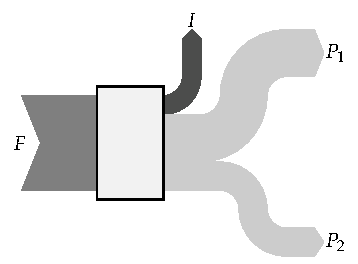
\includegraphics{reglaP.pdf}
  \end{minipage}
  \begin{minipage}[c]{0.45\linewidth}
    \centering
    \textbf{Rule P}
    \begin{equation*}
        \eta=\frac{P_1+P_2}{F}
    \end{equation*}
    \begin{equation*}
        k_{P,1}^*=k_{P,2}^*    
    \end{equation*}
  \end{minipage}
\end{center}
\begin{center}
  \begin{minipage}[c]{0.50\linewidth}
    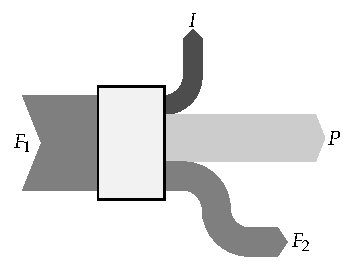
\includegraphics{reglaF.pdf}
  \end{minipage}
  \begin{minipage}[c]{0.45\linewidth}
    \centering
    \textbf{Rule F}
    \begin{equation*}
        \eta=\frac{P}{F_1-F_2}
    \end{equation*}
    \begin{equation*}
        k_{F,1}^*=k_{F_2}^*    
    \end{equation*}
  \end{minipage}
  \captionof{figure}{Cost allocation rules P and F in stream bifurcation}
  \label{fig:RulesFP}
\end{center}

These rules link  the concepts of the unit exergy cost, $k^*$, of the streams with the efficiency definition of the components, $\eta \equiv 1/k$, one-to-one, where $k$ is named the unit exergy consumption of the component. This is the essential message of the \emph{Theory of Exergy Cost}, which has been extensively used to assess the costs of many thermoeconomic/thermodynamic applications.

However, a number of questions have arisen. First, based on its definition, the exergy cost depends on the plant disaggregation scheme. In other words, it cannot render a precise value because it depends on the analyst choice. For instance, a chemical plant produces ethylene and electricity, which are not produced in the same process but in the same plant; hence, either $P$ or $F$ rule applies. Therefore, the formation and type of the streams and how much and where the exergy has been consumed in the process must be analyzed. This detailed analysis provides a productive structure to which the rules can be applied in practical terms. A more detailed definition is more precise; however, there is the risk of not having measured data that corroborate the sensitivity of the obtained costs to variations in these data. There are major discrepancies among practitioners regarding the definition of productive structures and the disaggregation method of the processes.

Second, the definition of exergy efficiency also depends on the analyst. For example, in a counter current heat exchanger, a stream becomes cooled, and another becomes heated. Hence, does the exchanger heat, cool, or both, and which stream assumes the production cost? Furthermore, not all components aim to save exergy (productive components). Certain other components in a plant are responsible for mitigating (the exergy of) wastes. Hence, it must be determined how to allocate costs to the components that process residues.
Third, exergy and its related cost depend on the chosen reference environment. However, the physical behavior of the plant does not depend on the analyst choice. Moreover, the right choice of the energy-like function for describing the plant might be in doubt: energy, exergy, (Gibbs) free energy, or any other generic function. 

Moreover, are the costs average costs or marginal costs? The exergy of a stream measures its potential with respect to a given environment, and the exergy cost measures how many irreversibilities have occurred in the manufacture of a stream or product. The exergy cost can be considered an “exergy backpack” or “exergy footprint” of a stream or product, i.e., the past exergy synopsis (history) of the stream, whereas its exergy is the future energy potential of such a stream or its remaining capacity to produce work. Finally, can the exergy costs predict future degradations or only past irreversibilities?

Despite these doubts, the analyst aims to obtain reasonable costs. Thus, it is necessary to disaggregate the system as far as common sense advises. Second, the definition of efficiency for each component requires caution. Third, choosing exergy is better than other energy-like functions because it provides a proxy for the locally usable energy. Fourth, the selected reference level for exergy must be realistic. Finally, the average costs should be useful in predicting how many additional resources compensate for the small system perturbations. While theory does not support these assumptions, practice does. The objective of this study is to revisit a general theory \cite{Valero1992a,Valero1992b}, for solving some of these questions and for providing a path for solving newly arising questions. 

%%%%%%%%%%%%%%%%%%%%%%%%%%%%%%%%%%%%%%%%%%
\section{On the Linearity of Cost: The Structural Theory of Thermoeconomics}
Any energy system that consumes resources and manufactures products can be characterized by a thermodynamic function $E$ of the generic type, $E = m (h-T_x\,s)$ where $m$ is the mass, $h$ the enthalpy, $s$ the entropy with respect to a certain reference, and $T_x$ the temperature to choose under certain conditions. When $T_x$ is zero, the function $E$ is the enthalpy; when $T_x$ is the ambient temperature, $E$ is the exergy; if $T_x$ is the temperature of the system, $E$ is the Gibbs function.
The mathematical behavior of any component $u$ can be described through functions of the type:
\begin{equation}
    \label{eq:gcf}
    E_i=f_i\left(\{x\},\{E_j\}\right) \qquad i\in\mathcal{E}_u
\end{equation}
where $i\in\mathcal{E}_u$ are the input flows of component $u$ and $j\in\mathcal{S}_u$ the output flows of component $u$, and $\{x\}$ is the set of its internal governing parameters, for instance, internal efficiencies, pressure relationships, temperature increases, geometric parameters, structural parameters, fluid dynamic parameters or heat transfer parameters.

On the other hand, the globally considered plant will receive some resources, be these $E_0$, defined as:
\begin{equation}
E_0=\sum_{j\in\mathcal{S}_0}{E_j}
\end{equation}
where $\mathcal{S}_0$ is the set of flows entering the plant (or leaving the environment).

If we identify the marginal unit cost with the derivative:
\begin{equation}
k_i^*\equiv\dpartial{0}{i}
\end{equation}
it satisfies evidently the following expresion for each and every component:
\begin{equation}
\dpartial{0}{j}=\sum_{i\in\mathcal{E}_u}{\dpartial{0}{i}\,\dpartial{i}{j}}
\label{eq:mcost}
\end{equation}

Note that in case of the flows entering the plant, it leads:
\begin{equation}
k_{j}^{*}=1 \qquad j\in\mathcal{S}_0
\end{equation}
which correspond to the external resources rule in the \emph{exergy cost theory}, or in other words, the cost of system's inputs are known and equal to its physical magnitude. 

Function \cref{eq:gcf} does generally not relate inputs and outputs linearly. Because the only degree of freedom is the choice of $T_x$ (i.e., the choice of energy, exergy, Gibbs function, or any other function), it is likely that the complexity of the equation cannot be reduced to a linear relationship.
However, such a continuous function allows for a Taylor series approximation. In addition, by choosing sufficiently small linear intervals, second-order terms can be discarded. The smaller the interval, the closer is the proposed behavior to reality. By applying this step, the following is obtained:
\begin{equation}
    E_i=\begin{dcases}
    \;\sum\limits_{j\in\mathcal{S}_u}{k_{ij}(x)\,E_j} \qquad &i\in\mathcal{E}_u \\
    \;\omega_i\;\text(const.) \qquad &i\in\mathcal{E}_0
    \end{dcases}
    \label{eq:echar}
\end{equation}
which relates the inputs and outputs in a linear way through parameters $k_{ij}$, which substitute the internal parameters for each identified component. Furthermore, the coefficients $k_{ij}$ take the name of technical production coefficients in the input–output theory \cite{Leontief1970}. They are the (average) unit consumption of resource $i$ necessary to produce stream $j$.

The advantage of a linear analysis is that it enables the understanding of many underlying assumptions in any cost allocation theory. Owing to the linearity, the coefficients $k_{ij}$ coincide with derivatives \emph{(ceteris paribus)} of the following type:
\begin{equation}
    k_{ij}\equiv\dpartial{i}{j}
\end{equation}
and
\begin{equation}
    E_i=\sum_{j\in\mathcal{S}_u}{\dpartial{i}{j}\,E_j} \qquad i\in\mathcal{E}_u
\end{equation}
Herein, this expression is called the \emph{component's characteristic equation}.

Moreover, the cost allocation is a basic application of the rule of the chain in the derivative calculation, and \cref{eq:mcost}, which is independent on the characteristic equations are linear or not, could be expressed as follow:
\begin{equation}
k_{j}^{*}=\sum_{i\in\mathcal{E}_u}{k_{ij}\,k_{i}^{*}}
\label{eq:kchar}
\end{equation}

The application of this equation explains the previously mentioned Rules $F$ and $P$ as a particular case. For example, a turbine (\cref{fig:turbine}) with the following defined efficiency is considered: 
\begin{center}
  \begin{minipage}[c]{0.50\linewidth}
   \centering
    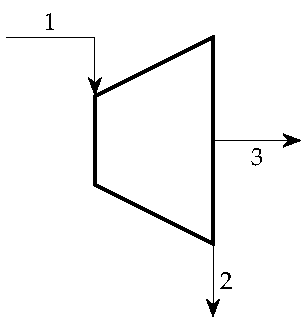
\includegraphics[scale=0.7]{turbine}
  \end{minipage}
  \begin{minipage}[c]{0.48\linewidth}
    \centering
    \begin{equation*}
        k=\frac{F}{P}=\frac{Ex_1 - Ex_2}{Ex_3}
        \label{eq:turb}
    \end{equation*}
    or
    \begin{equation*}
        Ex_1=Ex_2+k\,Ex_3
    \end{equation*}
  \end{minipage}
  \captionof{figure}{Conventional efficiency definition of a turbine, as an example of the Rule F application}
  \label{fig:turbine}
\end{center}

In what follows, it is assumed that the characteristic equation of the turbine coincides with the exergy definition of the turbine. In the simulations of the turbine for a reasonably small working interval, k can be considered constant. By applying the unit cost \cref{eq:kchar}, the costs of outputs 2 and 3 are obtained:
\begin{equation}
    k_3^*=k\,k_1^* \qquad\text{and}\qquad k_2^*=k_1^*
\end{equation}
Hence, the result is \emph{Rule F}, i.e., if a resource has not been totally consumed (stream 2), its unit cost is equal to that of the input resource (stream 1).                    

However, if a typical electric power distribution system is considered, its efficiency can be expressed as follows:
\begin{center}
  \begin{minipage}[c]{0.50\linewidth}
   \centering
    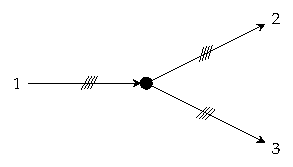
\includegraphics[width=0.8\linewidth]{distribucion}
  \end{minipage}
  \begin{minipage}[c]{0.48\linewidth}
    \centering
    \begin{equation*}
        k=\frac{F}{P}=\frac{Ex_1}{Ex_2+Ex_3}
        \label{eq:dist}
    \end{equation*}
    or
    \begin{equation*}
        Ex_1=k\,Ex_2+k\,Ex_3
    \end{equation*}
  \end{minipage}
  \captionof{figure}{Generic electric power distribution system as an example of application of Rule P.}
  \label{fig:distributor}
\end{center}

Again, it is assumed that the characteristic equation of the distribution system coincides with its exergy definition. If k is constant, applying the unit cost \cref{eq:echar} results in:
\begin{equation}
    k_2^*=k\,k_1^*     \qquad \text{and}\qquad    k_3^*=k\,k_1^*
\end{equation}
which explains why \emph{Rule P} applies; that is, the unit costs of the products of the same nature produced in the same process are equal.

In general, the disaggregation of the process in \cref{fig:genplant} can be described by the following system of characteristic equations \eqref{eq:egenplant}: 
\begin{figure}[H]
    \centering
    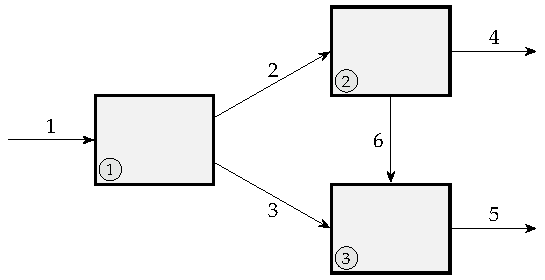
\includegraphics{genplant}
    \caption{Generic energy system}
    \label{fig:genplant}
\end{figure}

\begin{equation}
    \def\arraystretch{2.1}
    \left\{\begin{array}{l}
        E_1=k_{12}\,E_2 + k_{13}\,E_3 \\
        E_2=k_{24}\,E_4 + k_{26}\,E_6 \\
        E_3=k_{35}\,E_5\\
        E_4=\omega_3 \quad \text{(const.)}\\
        E_5=\omega_4 \quad \text{(const.)}\\
        E_6=k_{65}\,E_5
    \end{array}\right.
    \qquad
    \text{or}
    \qquad
    \left\{\begin{array}{l}
        E_1=\dpartial{1}{2}\,E_2 + \dpartial{1}{3}\,E_3 \\
        E_2=\dpartial{2}{4}\,E_4 + \dpartial{2}{6}\,E_6 \\
        E_3=\dpartial{3}{5}\,E_5\\
        E_4=\omega_4 \quad \text{(const.)}\\
        E_5=\omega_5 \quad \text{(const.)}\\
        E_6=\dpartial{6}{5}\,E_5
    \end{array}\right.
    \label{eq:egenplant}
\end{equation}
Subsequently, according to the rule of the chain of the derivatives, the following expressions are obtained:
\begin{equation}
    \def\arraystretch{2.1}
    \left\{\begin{array}{l}
       \dpartial{0}{1}=1 \\
       \dpartial{0}{2}=\dpartial{0}{1}\,\dpartial{1}{2} \\
       \dpartial{0}{3}=\dpartial{0}{1}\,\dpartial{1}{3} \\
       \dpartial{0}{4}=\dpartial{0}{2}\,\dpartial{2}{4} \\
       \dpartial{0}{5}=\dpartial{0}{3}\,\dpartial{3}{5} + \dpartial{0}{6}\,\dpartial{6}{5} \\
       \dpartial{0}{6}=\dpartial{0}{2}\,\dpartial{2}{6} \\
    \end{array}\right.
    \qquad
    \text{or}
    \qquad
       \left\{\begin{array}{l}
        k_1^* = 1 \\
        k_2^* = k_1^*\,k_{12} \\
        k_3^* = k_1^*\,k_{13} \\
        k_4^* = k_2^*\,k_{24} \\
        k_5^* = k_3^*\,k_{35} + k_6^*\,k_{65} \\
        k_6^* = k_2^*\,k_{26} \\
    \end{array}\right.
    \label{eq:kgenplant}
\end{equation}
\Cref{eq:echar} can be rewritten in the matrix form: 
\begin{equation}
    \vm{E}=\left[\vm{K}\right]\,\vm{E}+\vm{\Omega}
    \label{eq:mechar}
\end{equation}
where $\left[\vm{K}\right]$ is the matrix of unit consumption's, and $\vm{\Omega}$ the vector of system's outputs values, and \cref{eq:kchar} becomes:
\begin{equation}
    \vm{k}^* = \tm\left[\vm{K}\right]\,\vm{k}^* + \vm{k}_0^*
    \label{eq:mkchar}
\end{equation}
where $\vm{k}_0^*$ is the unit cost of the system's input flows.

\begin{equation*}
    \def\arraystretch{1.5}
    \left[\vm{K}\right]=\left[\begin{array}{cccccc}
    0 & k_{12} & k_{13} & 0 & 0 & 0 \\
    0 & 0 & 0 & k_{24} & 0 & k_{26} \\
    0 & 0 & 0 & 0 & k_{35} & 0 \\
    0 & 0 & 0 & 0 & 0 & 0 \\
    0 & 0 & 0 & 0 & 0 & 0 \\
    0 & 0 & 0 & 0 & k_{65} & 0
    \end{array}
    \right]
    \qquad
    \vm{\Omega}=\left[\begin{array}{c}
    0 \\
    0 \\
    0 \\
    \omega_4 \\
    \omega_5 \\
    0
    \end{array}
    \right]
    \qquad
    \qquad
    \vm{k}_0^*=\left[\begin{array}{c}
    1 \\
    0 \\
    0 \\
    0 \\
    0 \\
    0
    \end{array}
    \right]
\end{equation*}

Note that the matrix of the unit consumption $\left[\vm{K}\right]$ is common and transposed between \cref{eq:mechar,eq:mkchar}. \Cref{eq:mechar} is the \emph{primal} of the structure and \cref{eq:mkchar} is its dual. Every productive structure or linear input–output interpretation of a system exhibits a primal representation with a corresponding single dual and vice versa \cite{Boyd2004}. 

\Cref{fig:genplantr} shows the dual cost structure of system in \cref{fig:genplant}. While the arrows in the productive process point from the resources toward the products, the cost structure (or dual) point from the products toward the resources. The costs search for the origin (causa materialis), while the products search for the final objective (causa finalis). \cite{Valero1990d}.

\begin{figure}[ht]
    \centering
    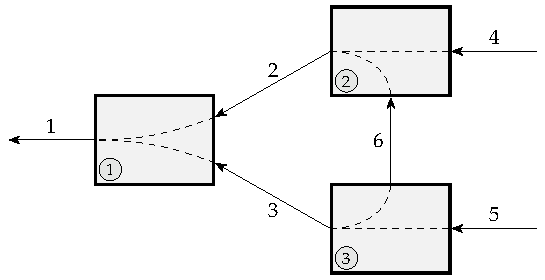
\includegraphics{genplantr}
    \caption{Dual cost structure of generic plant in \cref{fig:genplant}}
    \label{fig:genplantr}
\end{figure}

The cost of the productive structure is a conservative property, this is to say, the cost of the inputs of any component are entirely transferred among its outputs \cref{eq:costbal}. It is a mathematical consequence of the founded hypotheses:
\begin{equation}
    \sum_{i\in\mathcal{E}_u}{E_i^*}=\sum_{j\in\mathcal{S}_u}{E_j^*}
    \label{eq:costbal}
\end{equation}

For instance, the case of component \#1 is chosen, and the input equation:
\[
E_1=k_{12}\,E_2+k_{13}\,E_3
\] 
is combined with its output equations $k_2^*=k_{12}\,k_1^*$ and $k_2^*=k_{12}\,k_1^*$, consequently: 
\[
 k_1^*\,E_1 = k_2^*\,E_2+k_3^*\,E_3
\]

In general, applying \cref{eq:echar,eq:kchar} to \cref{eq:costbal} the cost balance is satisfied:
\begin{equation}
    \sum_{i\in\mathcal{E}_u}{k_i^*\,E_i}=\sum_{i\in\mathcal{E}_u}{k_i^*\,\sum_{j\in\mathcal{S}_u}{k_{ij}\,E_j}}=\sum_{j\in\mathcal{S}_u}{\left(\sum_{i\in\mathcal{E}_u}\,k_i^*\,k_{ij}\right)E_j}=\sum_{j\in\mathcal{S}_u}{k_j^*\,E_j}
\end{equation}
and the cost balance for the global plant, will be:
\begin{equation}
    E_0=\sum_{j\in\mathcal{S}_0}{E_j}=\sum_{i\in\mathcal{E}_0}{k_i^*\,E_i}
\end{equation}

Therefore, the plant's incidence matrix $\vm{A}$, can be defined as:
\begin{equation}
    a_{ij}=\begin{cases}
    \phantom{-}1 & \text{if}\qquad j\in\mathcal{E}_i \\
    -1 & \text{if}\qquad j\in\mathcal{S}_i \\
    \phantom{-}0 & \text{otherwise}
    \end{cases}
\end{equation}
hence, the analyzed case can be described as follows:
\begin{equation*}
    \vm{A}=\left[\begin{array}{rrrrrr}
    1 & -1 & -1 &  0 &  0 &  0 \\
    0 &  1 &  0 & -1 &  0 & -1 \\
    0 &  0 &  1 &  0 & -1 &  1
    \end{array}\right]
\end{equation*}

In general, the following expression holds:
\begin{equation}
    \vm{A} \cdot \vm{E}^{*} = \vm{0}
    \label{eq:mbalcost}
\end{equation}
and \cref{eq:mbalcost} shows the \emph{cost conservation equation}. It is a mathematical consequence of the founded hypotheses.

This result is quite remarkable because the following equations sumarize straightforwardly the Equilibrium Thermodynamics for open systems:
\begin{align}
    &\vm{A}\cdot\vm{M} = \vm{0} &\quad & \text{Mass Balance} \label{eq:a1} \\
    &\vm{A}\cdot\vm{H} = \vm{0} &\quad & \text{Energy Balance} \label{eq:a2}\\
    &\vm{A}\cdot\vm{Ex} = \vm{I} &\quad & \text{Exergy Balance} \label{eq:a3}\\
    &\vm{A}\cdot\vm{Ex^*} = \vm{0} &\quad & \text{Cost Balance} \label{eq:a4}
\end{align}
where \vm{M},\vm{H} and \vm{Ex} are the mass, enthalpy and exergy vectors of the material streams: $m_i$, $m_i\,h_i$ and $m_i(h_i-T_0\,s_i)$; if there are the heat flows: \emph{zero}, $Q$ and $Q(1-T_0/T)$; and \emph{zero}, $W$ , $W$ if there are working flows, respectively. Note the  parallelism with respect the cost equation \eqref{eq:mbalcost}. The presented structural theory explains the previously presented exergy cost theory.

\section{Outcomes}
The presented theory mitigates several important deficiencies of the conventional exergy costing theories. First, its results do not depend on a disaggregation scheme. For example, the system in \cref{fig:genplant} is aggregated into a single component \cref{fig:genplanta}.

\begin{figure}[h]
    \centering
    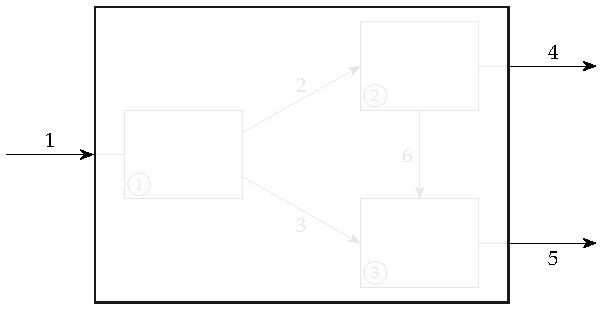
\includegraphics[scale=0.9]{genplanta}
    \caption{Aggregated system of \cref{fig:genplant}}
    \label{fig:genplanta}
\end{figure}
The physical behavior of the system remains (if linearized) the same under \cref{eq:gcf,eq:echar}. However, neither the \emph{Rule P} or \emph{F} can be applied between streams 4 or 5. In other words, $k_4^*$ is not equal to $k_5^*$, nor to $k_1^*$ .Therefore, the theory provides many hints how to explore the cost relationships and suggests that greater disaggregation schemes are required.

The main idea originates from the difference between the characteristic equation, and the efficiency equation (e.g. \cref{fig:turbine} or \cref{fig:distributor}). The former reflects the physical behavior of the component while the second is a definition, (i.e. an identity). The (linearized) characteristic equation of \cref{fig:genplanta} is expressed as follows:

Take, for instance, the case of , its (linearized) characteristic equation is of the type:
\begin{equation*}
    E_1=k_{14}\,E_4 + k_{15}\,E_5
\end{equation*}

Its efficiency equation could be of the following type:
\begin{equation*}
   Ex_{1} \equiv k\,Ex_{3}+Ex_4 
\end{equation*}

The similarity is evident; however, the more the analyst aggregates, the more deviates the physical behavior of the system from the definition. Note that the reference environment of the exergy depends on the practitioner choice, whereas \cref{eq:echar} should be independent.

The Structural theory \cite{Valero1992a,Valero1993} has been largely ignored in the study of different alternate rules for costing allocations, such as in the allocation of the costs of wastes, by-products, or co-products. This might be due to the difficulties of determining the fundamental equations of components as in \cref{eq:gcf} or their linearized equations, \cref{eq:echar}. Rather, the theory has been used to check the logics of rules $F$ and $P$.

Note that Odum's Emergy Analysis \cite{Odum1988,Brown1996} does not satisfy \eqref{eq:mbalcost} because it considers that when a biological system produces simultaneously two products, the same amount of solar energy is required for each product. This does not deny the idea of emergy; it simply states that this is not a regular cost.

In the same way, a non-linear theory does not satisfy \cref{eq:mbalcost} because the primal would be of the following type:
\begin{equation}
dE_i=\sum_j \dpartial{i}{j}\, dE_j,
\label{eq:dchar}
\end{equation}
rather than as \cref{eq:mbalcost}. However, \cref{eq:dchar} enables a generalization of the theory, For example, in \cite{Brown1996}, the costs are the Lagrange multipliers of an optimization of the plant.

The structural theory formally relates to the input-output theory \cite{Leontief1970}; however, \emph{the characteristic equation makes the difference because it deeply connects the thermodynamic behavior of an energy system to the stream costs such as in a transparent box}. Instead of the economic performance of highly aggregated economy sectors, their input–output flows are obtained outside the black boxes, which constitute each sector of the economy. In addition, the second law exergy analysis appears as a natural connection because it locates and accounts for irreversibilities occurring in a plant; thus, \emph{it relates the physical losses to the costs}. Note that “cost” is a concept that originates from economics, while “irreversibility” originates from thermodynamics. The structural theory can be considered a sought-after bridge between classical economics and physics. Thus, the term “thermoeconomics” is more appropriate than alternatives such as exergoeconomics \cite{Tsatsaronis2007}. 


\section{Drawbacks of Exergy?}
One important result of the structural theory is that any energy function of the type ${E=H-T_x\,S}$, may be used to assess different sets of costs. Thus, why should exergy that uses a fixed $T_0$ instead of a variable $T_x$ be considered? The most important objective of this study is to question the exergy directly to assess costs. 

Mythologizing exergy is not convenient, it only measures the number of times that a product is potentially equivalent to another. Therefore, the kilograms of natural gas; mass of steam at a certain temperature and pressure; and kinetic, magnetic, or mechanical energies are possible units for measuring exergy. Certainly, it does not reflect the product value. A broken glass has practically the same exergy as a new one, and the chemical exergy of gold is zero. Moreover, everybody would prefer 1 g diamond than 1 g pure graphite, even though they practically have the same exergy.

In addition, the manufacture of a continuous and broken thread costs the same exergy although the latter would not be saleable. Exergy reduces a probably irreducible object to a single numerical value. The color, taste, form, texture, or artistic impression (i.e., properties that human beings value) have no distinguishable exergy. The exergy and exergy cost are only a measure of reality, which should not supplant other possible analyses.

Can the concept of value be assessed by thermodynamics? Does it make sense to go beyond the exergy cost when it comes to knowing the cost of objects? It has been claimed many times that exergy is a measure of the quality of things, which is false; it is a measure of the energy imbalance that a system has with respect to a reference environment. It is a measure of the thermodynamic quality of energy and not of objects. Moreover, the quality specification is much more complex. A dose of carbon monoxide may have the same exergy as a certain amount of food; however, everybody knows which one to ingest or burn in a boiler. The same food can present a disgusting or an extraordinary aspect and contain the same amount of exergy. Based on the many possible examples, it seems strange to confuse exergy with quality.

Assessing quality requires many specifications such as the pressure, temperature, composition, height, and speed. Quality also depends on the context, whereas exergy does not. In general, thermodynamic equivalence is not a measure of the equivalence of values. Even circumstances and the moment make a thing seem more or less valuable. Researchers should distance themselves from neo-energeticism (or even better “exergeticism”), which regards exergy rather as a measure of the value of objects than as their monetary value. The exergy and exergy costs provide complementary information on the human footprint on Earth; ignoring them is as dangerous as extolling them as a unique instrument for managing the natural resources and environment.
 
Furthermore, the second law has not exhausted its message regarding exergy. The following equation:
\begin{equation}
   F - P = I + R
\label{eq:FPR}
\end{equation}
identifies product, waste, and what is (or is not) a usable resource. Certainly, every real-world process experiences an irreversibility. The Gouy–Stodola theorem relates the entropy generation to irreversibility:
\begin{equation}
    I = T_0\,S_g
\label{eq:gouystodola}
\end{equation}

Regardless of the way the quality of every flow, product, or service is defined (generalized exergy function), it is easier to identify the quantity. Thus, the magnitude of a property $X$ is always a product of its quantity $q_x$ multiplied by its specific quality $x$:
\begin{equation}
X=q_x\cdot x
\end{equation}                      

It would be interesting to determine the number of resources required to compensate for a deterioration of any component in a constant production for a set of quality specifications for each flow interacting in a system.

\section{The Relative Free Energy Function}
Before generalizing the problem, a simple case should be analyzed: for example, the expanding flow of a turbine produces work on the axis. In an $(h, s)$ diagram, \cref{fig:dt1}, the actual process evolves from state 1 to state 2. 
\begin{center}
	\begin{minipage}[c]{0.48\linewidth}
		\centering
		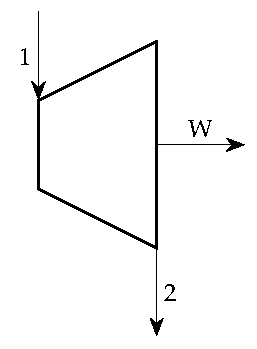
\includegraphics[scale=0.8]{turbinew}
	\end{minipage}
	\begin{minipage}[c]{0.48\linewidth}
		\centering
		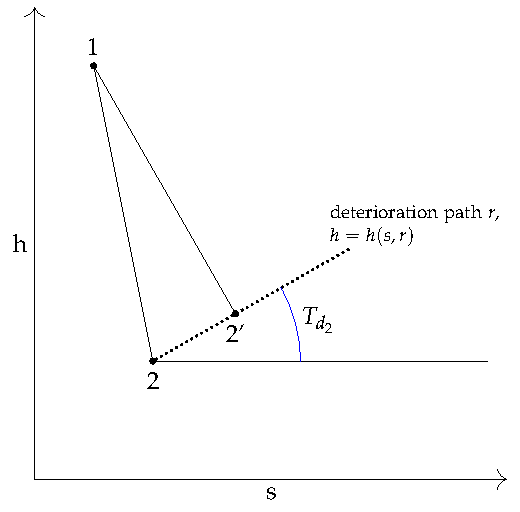
\includegraphics[scale=0.8]{dt1}
	\end{minipage}
	\captionof{figure}{The deterioration path of a turbine}
	\label{fig:dt1}
\end{center}

The energy and entropy balances of the process (first and second laws) are as follows:
\begin{align}
W=&\,m\left(h_1-h_2\right)\\
S_g=&\,m\left(s_2-s_1\right)
\end{align}

If the turbine degrades, at a rate equal to the specifications of the inflow \#1, an increase in the entropy generation evidently results in an increase in the amount of entering fuel (path 1) to keep the production constant. Owing to the degradation, the new state of the outflow \#2' is characterized by  ($h_{2'}$, $s_{2'}$).

A differential analysis under the conditions: $W$=const., $h_1$=const., and $s_1$=const., leads to the following expressions:
\begin{align}
\left(h_1-h_2\right) dm &= m \, dh_2\\
\left(s_1-s_2\right) dm + m \, ds_2 &= dS_g
\end{align}
Subsequently, the \emph{deterioration temperature} of flow \#2 is defined as a quotient:
\[
T_{d_2}\equiv dh_2/ds_2
\]
and the result is as follows:
\begin{equation}
\left(\frac{dm}{dS_g}\right)_r =\frac{T_{d_2}}{\left(h_1-h_2\right)-T_{d_2}\,\left(s_1-s_2\right)},
\label{eq:dt2}
\end{equation}
where $r$ is the deterioration path, as it shown is \cref{fig:dt1}.

\Cref{eq:dt2} is the mathematical expression of the existing relationship between any local degradation and the increase in associated resources if the production of the component should remain constant.

These equations and the function $\ell\equiv (h_1-h_2) - T_d (s_1 - s_2)$ were presented in \cite{Valero1992b}. Valero called it the \emph{relative free energy} (RFE), and $T_d$ the \emph{deterioration temperature} \cite{Royo1994,Royo1995}. The expression “relative free energy” originates from its similarity to the Gibbs free energy function. \Cref{eq:dt2} states that any deterioration process in an energy component has an associated $T_d$. This parameter possesses temperature dimensions even if it is not a measurable temperature; it can be calculated by measuring the quotient $dh_2/ds_2$ experienced by the output flow of the component.

The heat exchanger \cref{fig:dt2} experiences the same procedure  
\begin{center}
	\begin{minipage}[c]{0.48\linewidth}
		\centering
		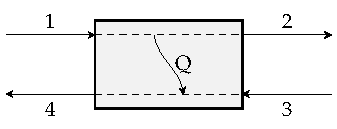
\includegraphics{heater}
	\end{minipage}
	\begin{minipage}[c]{0.48\linewidth}
		\centering
		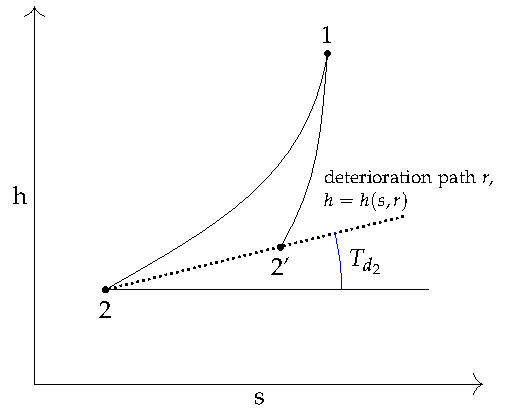
\includegraphics[scale=0.8]{dt2}
	\end{minipage}
	\captionof{figure}{Deterioration path of heat source in heat exchanger}
	\label{fig:dt2}
\end{center}

In that case, the enthalpy and entropy balances are written as follows: 
\begin{align}
m_1 \left(h_1 - h_2 \right) - m_3 \left(h_4 -h_3\right) &= 0 \\
m_1 \left(s_1 - s_2 \right) - m_3 \left(s_4 - s_3 \right) &= S_g 
\end{align}

If the heat source degrades, at equal to the specifications of the inflow \#1, an increase in the entropy generation results evidently in an increase in the amount of entering fuel \#1 to maintain a constant production; thus, $m_3$, $(h_3, s_3)$, and $(h_4, s_4)$ are constant. Owing to the degradation, the new state of outflow \#2' is characterized by $(h_{2'}, s_{2'})$.   

A differential analysis under these conditions leads to $(h_1,s_1)$ = constant:
\begin{align}
\left(h_1 - h_2\right) dm_1 = m_1 dh_2 \\
dS_g - \left(s_1 - s_2\right) dm_1 = - m_1 ds_2 
\end{align}

The dissipation temperature of flow \#2 is defined as a quotient:
\[
	T_{d_2}\equiv -\frac{dh_2}{ds_2}>0
\]
and subsequently \cref{eq:dt2} is also satisfied.

According to the second law, $dS_g$ is always positive; therefore, more fuel must be used to obtain the same product, and $dm > 0$. Because $T_{d,2}$ is positive, the term $(h_2-h_1 )-T_{d,2} (s_2-s_1 )$ must be positive; in other words, $T_{d,2} (s_1-s_2)$ is always greater than $(h_1-h_2)$.

\section{h-s Deterioration(s) Path(s) of an Energy System}
Man-made energy systems transform the energy flows one into another flows with a purpose. Commonly, the name of a component describes its function: a boiler boils water, a condenser condenses, and a heat exchanger exchanges heat. The understanding of how nature behaves is the basis of the component design. The entering flow performs a purposive path through which its thermodynamic properties change progressively until the flow exits the component. This path is never strictly determined, either because of possible changes in the quantity/quality of the entering flow or because of changes in the behavior of the component itself. This path variation results in a change in the properties of the exiting flow with respect to its design conditions. There are as many new exit states as causes of change, which are called “malfunctions” and are classified into two categories: intrinsic and induced \cite{Valero2004c,Valero1999c,Torres1999}. The term “intrinsic” refers to the internal deterioration of the component; the term “induced” refers to its off-design conditions (not the optimal operating conditions). A good component design foresees most of these off-design conditions. Literature and some manufacturers provide governing equations and control parameters based on semi-empirical models of the machines.

For a given deterioration cause $r$ of an energy component, either intrinsic or induced, a geometric path in the $h-s$ plane of the possible exit flow states can be identified. Let $h_{2'}=h_{2'}(s_{2'}, r)$ to be the function describing this dissipation path of the exiting flow, as in \cref{fig:dt1}, where:
\begin{description}
	\item[$1 \longrightarrow 2:$]  is the design path of the stream in the component.
	\item[$1 \longrightarrow 2':$] is the stream path after the component deterioration.
	\item[$2 \longrightarrow 2':$] is the dissipation path of the exiting stream $h_{2'} = h_{2'} (s_{2'}, r).$
\end{description}

The function $h_{2'}=h_{2'} (s_{2'}, r)$ ) can be regarded as the mathematical description of the effects on the exiting flow caused by the component deterioration cause $r$. This function always exists for a given differential malfunction interval. Moreover, under actual machine conditions, this function is a composite curve of the different paths caused by the concurrent deteriorations acting simultaneously on the component \cite{Valero2004c}. The next section focuses on this function.

\section{The Legendre Transform of a Deterioration Path}
For each deterioration cause, $r$, the existence of a function $h = h(s)$ of the exiting flow can be assumed, which can be described in the $h-s$ plane with the conventional point geometry or Plücker line geometry for strictly convex functions as a convolution of the tangents of the original curve. This technique is named the \emph{Legendre transform} of the function $h = h(s)$ and is widely used in classical thermodynamics \cite{Callen1985,Alberty2001}.

\begin{figure}[ht]
	\centering
	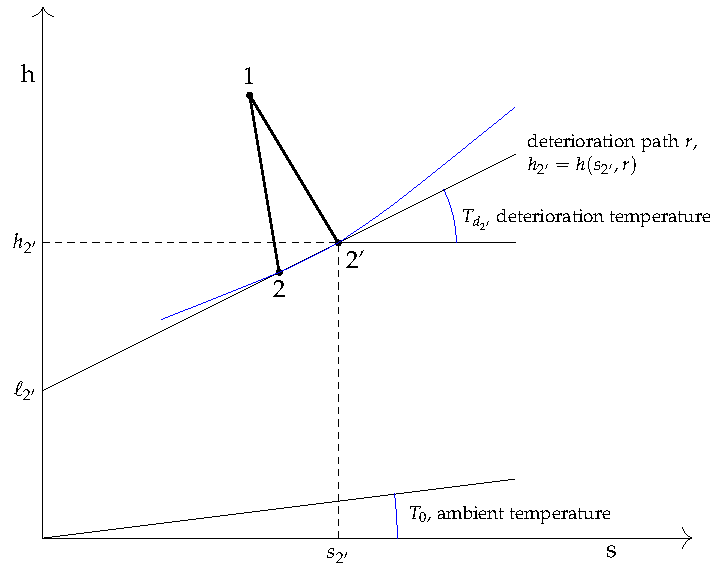
\includegraphics[scale=0.78]{rfe.pdf}
	\caption{Geometric representation of the relative free energy and deterioration temperature}
	\label{fig:rfe}
\end{figure}

\Cref{fig:rfe} shows that the intercept on the $h-axis$ of the tangent line is $\ell$ with slope $T_d$:
\[
T_d=\frac{h-\ell}{s}
\]
or
\begin{equation}
\ell=h-T_d\,s \qquad \text{i.e.} \qquad \ell=\ell(T_d)
\label{eq:lgdr}
\end{equation}

\Cref{eq:lgdr} is the \emph{Legendre transform} of the deterioration path $h_{2'}=h_{2'}(s_{2'},r)$. In fact, pairs of $(\ell_{2'} , T_{d,2'})$ for each exit state, \#2', of the component provide the same information as pairs $(h_{2'},s_{2'}$). Because the relationship  $\ell_{2'} = \ell_{2'}(T_{d,2'})$ is mathematically equivalent to the relationship $h_{2'} = h_{2'} (s_{2'}, r)$, it can also be considered the description of the deterioration path. More in general, $h_r=h_r (s_r)$, is the deterioration function in the \emph{h-representation}; whereas $\ell_r = \ell_r(T_d,r)$ is the deterioration function in the \emph{l-representation} . In other words, $\ell_r$ and $T_{d,r}$ , are inseparable in a deterioration path, $r$, such as $h_r$ and $s_r$ do. Note also that $h$ and $s$ do not represent absolute values because they refer $h_0$ and $s_0$ values. Unless otherwise stated $h$ and $s$ represent $(h-h_0)$ and $(s-s_0)$.

The deterioration temperature, $T_d$, is not a physical temperature; ; it is a parameter and derivative with temperature dimensions:  
\begin{equation}
T_d=\left(\frac{dh}{ds}\right)_r
\end{equation}      

It can be interpreted as the entropic cost of the dissipation. The greater Td, the lower is the relative free energy of the exiting flow.
Well-known contributors to technical thermodynamics such as Baehr \cite{Baehr2005,Baehr1979} have defined the “friction work” or “loss work” for an expander as follows: 
\begin{equation}
	dW_r=T_d\,dS_g
\end{equation}

This loss work is energy that has not been dissipated into the environment at $T_0$ and contributes to the degradation of the exiting flow of the expander. It increases the enthalpy and entropy of the exiting stream and reduces the work produced by the turbine, thereby decreasing its efficiency.

Another important antecedent was the work of Alefeld \cite{Alefeld1988}, who worked on heat pumps and refrigeration systems: he questioned the use of the reference ambient temperature $T_0$ instead of a variable temperature $T_x$ associated with the equipment. In particular, he proposed for the case of a condenser, that this temperature $T_x$ be equal to that of the condenser vacuum, $T_{vac}$. Alefeld was highly criticized by the community of exergy practitioners, because the holistic vision that exergy provides was lost in his theory. This article is a recognition to his work because mathematical proofs are stronger than reasonable assumptions.

\section{Relationship Between Exergy and Relative Energy Function Transform} 
The relative free energy function $\ell$ represents the local free energy conditioned by the dissipation path, $r$. It is an intensive property, and its corresponding extensive property: 
\begin{equation}
\Lgdr = m\,\ell
\end{equation}                                                
is the amount of energy of the exiting stream in a fuel or a product of the type $E_1-E_2$, which is not affected by the deterioration of the component. This is because when the exit flow changes its state owing to the deterioration, $h$ and $s$, vary by following the path $h_r = h_r (s_r)$. Consequently, the following expression is obtained:
\begin{equation}
d\ell = dh_r - \left(\frac{dh}{ds}\right)_r\, ds_r = 0 \qquad  \text{or} \qquad      \ell = const.
\end{equation}

In addition, the function $h_r = h_r(s_r)$ is neither a straight curve not has it a slope $T_0$. Therefore, $\ell$, exceptionally coincides with the specific exergy of the flow, and the exergy increase in the output stream in the turbine is $(h_{2'} - h_2) - T_0 (s_{2'} - s_2)$ or $ex_1-ex_2$. 

In the example of the turbine, if $F-P=I$, a differential analysis under the conditions $(h_1,s_1)$ and $W=P$ constants, lets:
\begin{equation}
dF=dI=T_0\,dS_g
\end{equation}
or
\begin{equation}
(h_{2'}-h_2)-T_0\,(s_{2'}-s_2)\,dm=T_0\,dS_g
\end{equation}
Therefore, the following expression is obtained:
\begin{equation}
dF=T_0\,dS_g=dW_r \frac{T_d}{T_0}
\end{equation}
and combining it with \cref{eq:dt2}, results in the following equations:
\begin{equation}
\left(\frac{dm}{dS_g}\right)_r = \frac{T_0}{ex_2'-ex_2}=\frac{T_{d,2}}{\ell_1-\ell_2}
\label{eq:dmsg}
\end{equation}

Consequently, function $\ell$ becomes more familiar. \Cref{eq:dmsg} presents the relationship between the increase in the entropy generation in a process in which a stream performs an activity; the amount of required additional resources depends on the following specifications: 
\begin{itemize}
	\item Constant quality of the entering resource, and
	\item Constant quality and quantity of the production,
\end{itemize}
Therefore, \cref{eq:dmsg} becomes as follows:
\begin{equation}
\left(\frac{dm_{in}}{dS_g}\right)_r = \frac{T_{d,2}}{\ell_1-\ell_2}
\end{equation}

This expression shows that the second law has not yet said the last word regarding the relationship between the quantity, quality, cost and irreversibility. 

In general, the reason of why $T_d$ instead of $T_0$ , stems from the fact that the additional degraded energy not used in producing the product becomes part to the exiting streaming instead of going directly to the environment at $T_0$. Then, $dh_2$ and $ds_2$ are always positive and the value of $T_d$ depends on how great the additional irreversibility is created. Such interpretation of $T_d$, allows understand that, its lowest attainable value is $T_0$, while it has no superior limits. 
Note also that if $T_d$ is greater than $T_0$, then $ex_i$ is always greater than $\ell_i$.

In other words, the deterioration lowers the free energy of the exiting stream. As this deterioration always relates to some component, this is why we name this function the relative free energy. In the same way that the Gibbs free energy relates to some chemical reaction, the RFE relates to some component deterioration in a system.

\section{Towards a New Diagnosis Theory of Energy Systems}
The key problem of diagnosis of energy systems stems in how to assess, as precisely as possible, the relationship between local irreversibilities and additional consumption of resources. At constant production, a local irreversibility needs additional resources to compensate it, but also modifies the exiting streams, affecting downstream enthalpies and entropies and eventually the upstream ones, if recycling. 
A certainty derives from the Second Law: Any inefficiency in a process increases the entropy generation. This means that any mechanical, thermal or chemical loss generates entropy and reduces efficiency. However, any efficiency decrease means more amount resources (at equal quality) to get the same product. 
If one knows the amount of local resources needed to compensate a local deterioration, $r$, i.e.
\[
\left(\frac{\partial m_{local}}{\partial S_g}\right)_r
\] 
and knows how the global system's resources is related with local resources, i.e.
\[
\left(\frac{\partial m_{global}}{\partial m_{local}}\right)_r
\]
one may have a new theory of energy system diagnosis. We will present this theory with due examples in a following paper, however, an early analysis was published in \cite{Royo1997}.

\section{Conclusions}
The definition of efficiency plays a fundamental role in the process of calculating average exergy costs. So efficiency and cost became closely linked. In such a way the \emph{Theory of Exergy Cost} \cite{Valero1986a,Lozano1993} was extensively used to assess costs on many thermoeconomic/thermodynamic applications. However, the exergy cost depends on the plant disaggregation scheme. It is necessary to look after “the cost formation process”, by searching how much exergy has been consumed in the processes and where they have consumed it. The result of this activity is a given productive structure. However, if exergy depends on a chosen reference state, exergy efficiencies and their closely related costs will depend on such selection. Notwithstanding, any deterioration that increases entropy generation results in an additional expense of resources used to produce the same product. Both, the entropy increase and the additional resources are measurable and free from analyst selections. Therefore, something fails in the conventional theory. 

The use of exergy instead of enthalpy or the Gibbs function for obtaining costs increase the overall, coherent and systematic view of a set of stream costs in a productive structure. To what extent one could use these costs to assess component malfunctions? In other words, can average costs be used as marginal costs?

The exergy cost is the “exergy backpack”, “embodied exergy” or the “exergy footprint” of a commodity; in fact, Szargut named it as “cumulative exergy consumption” i.e. its “past” characterization (history), while exergy is the potential energy of such a commodity, or its remaining capacity for doing something. Can average costs predict future degradations or only past irreversibilities? 
The purpose of Thermoeconomics is to obtain a coherent and significant set of costs in a given structure. That is because its applications are directed towards the optimization and diagnosis of productive structures. Therefore, the costs of internal streams are quite important to analyze the behavior of the system. Consequently, internal costs ought to be as sensitive as possible to system degradations. A theory that would provide exact costs would be the objective of thermoeconomic diagnosis. In fact, one can obtain the costs of final products, without performing very detailed analyses. In other words, in no way Thermoeconomics, as it is already known, is far from being finished. Moreover, the analyst needs to look for the “process of formation of cost of wastes” not mentioned here even when some ideas developed here could be used to clarify it.

This paper presents a General Theory of (linear) Costing, demonstrating and answering questions like:
\begin{itemize}
	\item To what extent the linear characteristic equation \eqref{eq:echar} a component can be conformed to its efficiency definition, $F - k\, P = 0$~? 
	In fact, exergy efficiency must be coherent with the component's design purpose, but one designs machines by observing the behavior of nature. So what is first, efficiency or nature?
	\item Why the F and P rules, or any other costing proposal may be either rational or not under a given disaggregation scheme.
	\item Under a set of conditions, we may say that the exergy costs balances are the mathematical dual of exergy balances and vice versa. The exergy cost and the exergy are like specular images of the same entity.
	\item To what extent the Exergy Cost Theory provides reliable results or not. Are exergy costs natural costs?
	\item A compact vision of current day Thermoeconomics/Exergoeconomics under the equations \cref{eq:a1,eq:a2,eq:a3,eq:a4}
	\item A costing theory applicable to any thermodynamic function like, enthalpy, Eexergy, Gibbs free rnergy or any other.
	\item In analyzing this last point, we proposed a new Thermodynamic function, called the \emph{relative free energy}, $\ell$ , and introduced a new parameter $T_d$ called deterioration temperature due to a component’s deterioration cause $r$ ,characterized by a thermodinamic trajectory $h=h(s, r)$ describing the effects on the exiting stream. 
	\item The exact equation \eqref{eq:dt2} in a turbine (and similarly in a heat exchanger or in any mass stream crossing an equipment) and its relationship with the exiting exergy stream \cref{eq:dmsg}.
	\item The Legendre transform of the deterioration path, $h_2=h_2 (s_2, r)$ is the relationship  
	$\ell_2 = \ell_2(T_{d,2} , r)$. In other words, the pairs  $\ell_r$ and $T_{d,r}$, are so inseparable in a deterioration path, $r$, as the pairs $(h_r,s_r)$ do.
	\item The general formula \eqref{eq:dmsg} applies for different flowing streams in energy systems under a given deterioration path, $r$. A given component may have several deterioration paths, not only one. Therefore, the concept of component malfunction need be associated with that of deterioration paths.	
\end{itemize}

This theory sketched here opens new fields of knowledge, since new questions appear:  Is exergy the best thermodynamic function when diagnosing systems? Why $T_0$ needs to be the same for each component of a given structure? Can we use this theory to assess objective average costs of deteriorations free from assumptions? The deterioration behavior of an energy system relates with internal marginal costs while exergy costs with history. Should we change our definitions of efficiency under the light of the relative free energy function? Etc. Even if described early in the nineties, all these ideas are tools for future, \cite{Naredo2000}. Cost is a measure of expended resources to produce something, then, costing with the Relative Free Energy instead of Exergy would open a new field of a more precise theory of Thermoeconomics. We presently work in such ideas.
%%%%%%%%%%%%%%%%%%%%%%%%%%%%%%%%%%%%%%%%%%
\vspace{12pt}
%%%%%%%%%%%%%%%%%%%%%%%%%%%%%%%%%%%%%%%%%%

\authorcontributions{Ideas, formulation of overarching research goals and aims, creation of models, writing of the initial draft, A.V.; verification of the overall reproducibility of results, C.T.; preparation of the published work specifically data presentation, C.T.} 
%%%%%%%%%%%%%%%%%%%%%%%%%%%%%%%%%%%%%%%%%%

\acknowledgments{My special thanks to Dr. Jean-Noël Jaubert who invited me to give a lecture at the Journées de exergie, Nancy, 22-23 Nov, 2018, and Prof. Michel Feidt who invited me to write the paper. They challenged me to explain and up-to-date this general theory of Relative Free Energy, that has a great explanatory power but was sleeping for a number of years.}
%%%%%%%%%%%%%%%%%%%%%%%%%%%%%%%%%%%%%%%%%%
\conflictsofinterest{The authors declare no conflict of interest. } 
%%%%%%%%%%%%%%%%%%%%%%%%%%%%%%%%%%%%%%%%%%
\reftitle{References}
\begin{thebibliography}{99}
	\providecommand{\natexlab}[1]{#1}
	\bibitem{Nancy2018}
	Valero, A.
	\newblock The duality between exergy efficiencies and exergy costs. The Structural Theory and the Relative Free Energy function.
	\newblock Journées sur le thème de l'éxergie, Nancy. France Nov. 22-23, 2018. 
	\newblock {\changeurlcolor{black}\url{https:/www.sfgp.asso.fr/journees-thematiques-exergies-22-23-novembre-2018} (accessed, Dec, 2019)}
	
	\bibitem[Valero and Lozano(1992)]{Valero1992a}
	Valero, A.; Lozano, M.
	\newblock A general theory of thermoeconomics: Part I. Structural Analysis.
	\newblock  ECOS '92 International Symposium, 1992, pp. 137--145.
	
	\bibitem[Valero and Lozano(1992)]{Valero1992b}
	Valero, A.; Lozano, M.
	\newblock A general theory of thermoeconomics: Part II. The relative free energy
	function.
	\newblock  ECOS '92 International Symposium,  1992, pp. 147--154.
	
	\bibitem[Valero \em{et~al.}(1986)Valero, Lozano, and Muñoz]{Valero1986a}
	Valero, A.; Lozano, M.; Muñoz, M.
	\newblock A general theory of exergy saving. I. On the exergetic cost.
	\newblock {\em Computer-aided engineering and energy systems: second law
		analysis and modelling} {\bf 1986}, {\em 3},~1--8.
	
	\bibitem[Morris and Szargut(1986)]{Morris1986}
	Morris, D.R.; Szargut, J.
	\newblock Standard Chemical Exergy of Some Elements and Compounds on the Earth
	Planet.
	\newblock {\em Energy} {\bf 1986}, {\em 11},~733--755.
	
	\bibitem[Szargut \em{et~al.}(1988)Szargut, Morris, and Steward]{Szargut1988}
	Szargut, J.; Morris, D.R.; Steward, F.
	\newblock {\em Exergy analysis of Thermal, Chemical, and Metallurgical Processes}; Hemisphere: New York,  1988.

	\bibitem[Lozano and Valero(1993)]{Lozano1993}
	Lozano, M.A.; Valero, A.
	\newblock Theory of the exergetic cost.
	\newblock {\em Energy} {\bf 1993}, {\em 18},~939--960.
	
	\bibitem[Tsatsaronis(2007)]{Tsatsaronis2007}
	Tsatsaronis, G.
	\newblock Definitions and nomenclature in exergy analysis and exergoeconomics.
	\newblock {\em Energy} {\bf 2007}, {\em 32},~249--253.
	
	\bibitem[Leontief(1970)]{Leontief1970}
	Leontief, W.
	\newblock Environmental repercussions and the economic structure: An input--output approach.
	\newblock {\em Review of Economics and Statistics} {\bf 1970}, {\em 52},~262--271.
	
	\bibitem[Boyd and Vandenberghe(2004)]{Boyd2004}
	Boyd, S.; Vandenberghe, L.
	\newblock {\em Convex {O}ptimization}; Cambridge University Press,  2004.
	
	\bibitem[Valero \em{et~al.}(1990)Valero, Carreras, Torres, and
	Lozano]{Valero1990d}
	Valero, A.; Carreras, A.; Torres, C.; Lozano, M.A.
	\newblock On {C}ausality in {O}rganized {E}nergy {S}ystems (parts {I}, {II} and
	{III}).
	\newblock  A Future for Energy, FLOWERS 1990,  1990, pp. 387--420.
	
	\bibitem[Valero \em{et~al.}(1993)Valero, Serra, and Lozano]{Valero1993}
	Valero, A.; Serra, L.; Lozano, M.
	\newblock Structural theory of thermoeconomics.
	\newblock  American Society of Mechanical Engineers, Advanced Energy Systems
	Division (Publication) AES; Richter, H.J., Ed. The American Society of
	Mechanical Engineers,  1993, Vol.~30, {\em H00874}, pp. 189--198.
	
	\bibitem[Odum(1988)]{Odum1988}
	Odum, H.
	\newblock Self-organization, transformity, and information.
	\newblock {\em Science} {\bf 1988}, {\em 242},~1132--1139.
	\newblock
	doi:{\changeurlcolor{black}\url{10.1126/science.242.4882.1132}}.
	
	\bibitem[Brown and Herendeen(1996)]{Brown1996}
	Brown, M.; Herendeen, R.
	\newblock Embodied energy analysis and EMERGY analysis: A comparative view.
	\newblock {\em Ecological Economics} {\bf 1996}, {\em 19},~219--235.
	\newblock
	doi:{\changeurlcolor{black}\href{https://doi.org/10.1016/S0921-8009(96)00046-8}{\detokenize{10.1016/S0921-8009(96)00046-8}}}.
		
	\bibitem[Royo(1994)]{Royo1994}
	Royo, J.
	\newblock Las ecuaciones caracteristicas de los sistemas térmicos. {L}a
	energía libre relativa.
	\newblock PhD thesis, Universidad de Zaragoza. Spain,  1994.
	
	\bibitem[Royo and Valero(1995)]{Royo1995}
	Royo, J.; Valero, A.
	\newblock Towards a unified description of the energy behavior of
	thermomechanical systems.
	\newblock  Analisys and Improvement of Energy Systems; Krane, R.J., Ed.,  1995,
	Vol.~35, pp. 127--134.
	
	\bibitem[Valero \em{et~al.}(2004)Valero, Correas, Zaleta, Lazzaretto, Verda,
	Reini, and Rangel]{Valero2004c}
	Valero, A.; Correas, L.; Zaleta, A.; Lazzaretto, A.; Verda, V.; Reini, M.;
	Rangel, V.
	\newblock On the thermoeconomic approach to the diagnosis of energy system
	malfunctions Part 2. Malfunction definitions and assessment.
	\newblock {\em Energy} {\bf 2004}, {\em 29},~1889--1907.
	
	\bibitem[Valero \em{et~al.}(1999)Valero, Torres, and Lerch]{Valero1999c}
	Valero, A.; Torres, C.; Lerch, F.
	\newblock Structural Theory and Thermoeconomic Diagnosis. Part III: Intrinsic and Induced Malfunctions.
	\newblock  Proceedings of the ECOS'99,  1999.
	
	\bibitem[Torres \em{et~al.}(1999)Torres, Valero, Serra, and Royo]{Torres1999}
	Torres, C.; Valero, A.; Serra, A.; Royo, J.
	\newblock Structural Theory and Thermoeconomic Diagnosis. Part I: On
	Malfunction and Dysfunction Analysis.
	\newblock  Proceedings of the ECOS'99; The American Society of Mechanical
	Enegineers: Tokyo, Japan,  1999; pp. 368--373.
	
	\bibitem[Callen(1985)]{Callen1985}
	Callen, H.B.
	\newblock {\em Thermodynamics and an {I}ntroduction to {T}hermostatistics},
	second ed.; Wiley,  1985.
	
	\bibitem[Alberty(2001)]{Alberty2001}
	Alberty, R.
	\newblock Use of Legendre transforms in chemical thermodynamics: (IUPAC
	Technical Report).
	\newblock {\em Pure and Applied Chemistry} {\bf 2001}, {\em 73},~1349--1380.
	\newblock
	doi:{\changeurlcolor{black}\href{https://doi.org/10.1351/pac200173081349}{\detokenize{10.1351/pac200173081349}}}.
	
	\bibitem[Baehr(2005)]{Baehr2005}
	Baehr, H.D.
	\newblock {\em Themodynamik}; Springer, 2005.
	
	\bibitem[Dieter(1979)]{Baehr1979}
	Dieter, B.H.
	\newblock {\em Tratado moderno de termodinámica. {T}eoría y aplicaciones
		técnicas}; Montesó,  1979.
	
	\bibitem[Alefeld(1988)]{Alefeld1988}
	Alefeld, G.
	\newblock Problems with the exergy concept (or the missing {S}econd {L}aw).
	\newblock {\em IEA Heat Pump Newsletter} {\bf 1988}, {\em 6},~19--23.
	
	\bibitem[Royo \em{et~al.}(1997)Royo, Valero, and Zaleta]{Royo1997}
	Royo, J.; Valero, A.; Zaleta, A.
	\newblock The dissipation temperature: A tool for the analysis of malfunctions
	in thermomechanical systems.
	\newblock {\em Energy Conversion and Management} {\bf 1997}, {\em
		38},~1557--1566.
	
	\bibitem[Valero(2000)]{Naredo2000}
	Valero, A.
	\newblock El marco termodínamico para iluminar la sociedad actual. In {\em
		Economía, ecología y sostenibilidad en la sociedad actual}; Naredo, J.M.;
	Parra, F., Eds.; Siglo XXI de España Editores,  2000; pp. 69--75.
	
\end{thebibliography}
\end{document}
